\chapter{Results}\label{chap:Results}


\section{Performance of the RRT* Algorithm}

In this master thesis, the performance of the RRT* algorithm itself was not improved but the parameters were tuned to serve the nonlinear optimization in an optimal manner.\newline
As mentioned in section \ref{sec:RRTstar}, the calculation time of the RRT* algorithm is mainly defined by the "rewiring" and therefore by the user specified parameter $\gamma$ (used in equation \ref{equ:ballradius}). A good straight line solution, whereas good means a small length of the straight line solution, does not necessarily lead to a good polynomial trajectory. The influence of the user specified parameter $\gamma$ on the final trajectory and the corresponding calculation time is evaluated in this section. \newline
Please call to mind that a small $\gamma$ parameter means little rewiring and a big $\gamma$ parameter means lots of rewiring. The impact of the $\gamma$ parameter can be looked up in figure \ref{pic:smallGamma} and figure \ref{pic:smallBBX}.\newline

\begin{figure}[H]
   \centering
   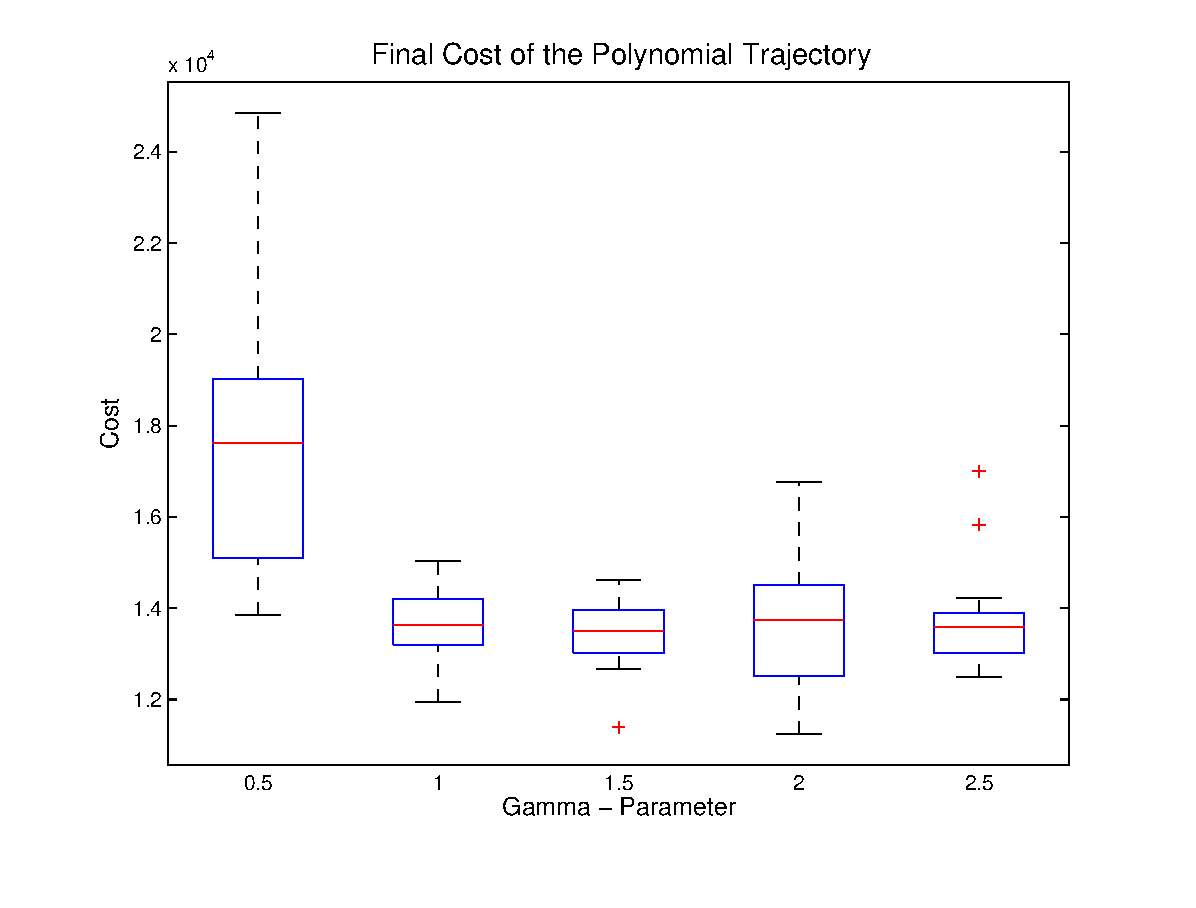
\includegraphics[trim = 14mm 10mm 15mm 0mm,clip,width=0.8\textwidth]{pics/boxplot1.eps}
   \caption{The $x$-axis depicts different $\gamma$ parameters and the $y$-axis depicts the final cost of the polynomial trajectory. The red mark illustrates the median. }
   \label{pic:boxplot}
\end{figure}

Figure \ref{pic:boxplot} depicts the boxplot for different $\gamma$ parameters. Each dataset consists of 15 measurements. On each box, the central mark is the median, the edges of the box are the 25th and 75th percentiles, the whiskers extend to the most extreme
datapoints the algorithm considers to be not outliers, and the outliers are plotted individually. \newline





It becomes apparent that the small amount of rewiring associated with $\gamma = 0.5$ is to little to obtain a good polynomial trajectory. The 4 remaining datasets have a similar performance in terms of the final trajectory cost. \newline

The total computational times for the five different $\gamma$ parameters are depicted in figure \ref{pic:boxplot_time}. The total computational time is the combined duration of the RRT* algorithm and the nonlinear optimization.  In contrast to the final cost, the total computational times for $\gamma = 1 $, $\gamma = 1.5$, $\gamma = 2$ and $\gamma = 2.5$ are distinct. 

\begin{figure}[h]
   \centering
   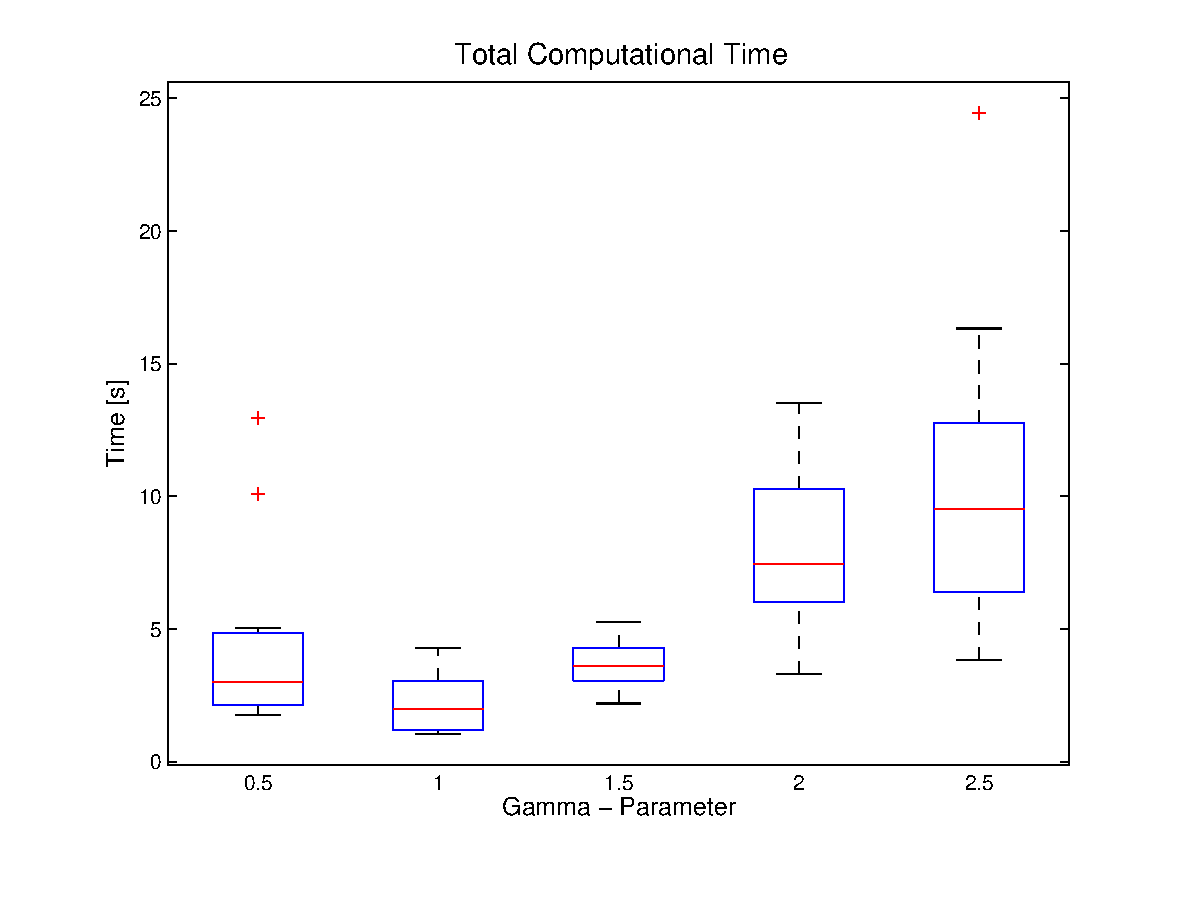
\includegraphics[trim = 14mm 10mm 15mm 0mm,clip,width=0.8\textwidth]{pics/boxplot_time.eps}
   \caption{The $x$-axis depicts different $\gamma$ parameters and the $y$-axis depicts the total computational time. The red mark illustrates the median.}
   \label{pic:boxplot_time}
\end{figure}

Figure \ref{pic:boxplot_time} shows that the computational time increases significant if $\gamma$ is larger than 1.5. This is simply because the RRT* algorithm needs more time for rewiring. Furthermore, $\gamma = 0.5$ (which is not a good choice sine the final cost is too high) has 2 outliers. In this 2 cases the straight line solution is not enough target-orientated and multible vertex extensions are required to obtain a collision-free trajectory. \newline

Combining the results from figure \ref{pic:boxplot} and figure \ref{pic:boxplot_time}, a $\gamma$ parameter in the range of 1 to 1.5 lead to the best performance.




\section{Performance of NLopt}

To test the performance of NLopt, a nonlinear optimization library, trajectories of different length were optimized. Figure \ref{pic:differentGoal} depicts a start vertex and 6 different goal vertices. The figure is in bird's eye perspective and shows a crossing of different hallways. The blue cells represents the floor and the green cells represents the walls. 
 In some of the hallways, there are objects blocking (part of) the way. This passages are tagged with "Bottleneck". Please note that other passages which may look like a bottleneck, such as the top right corner, are not blocked. The green boxes in this passage are part of the ceiling.

\begin{figure}[H]
   \centering
   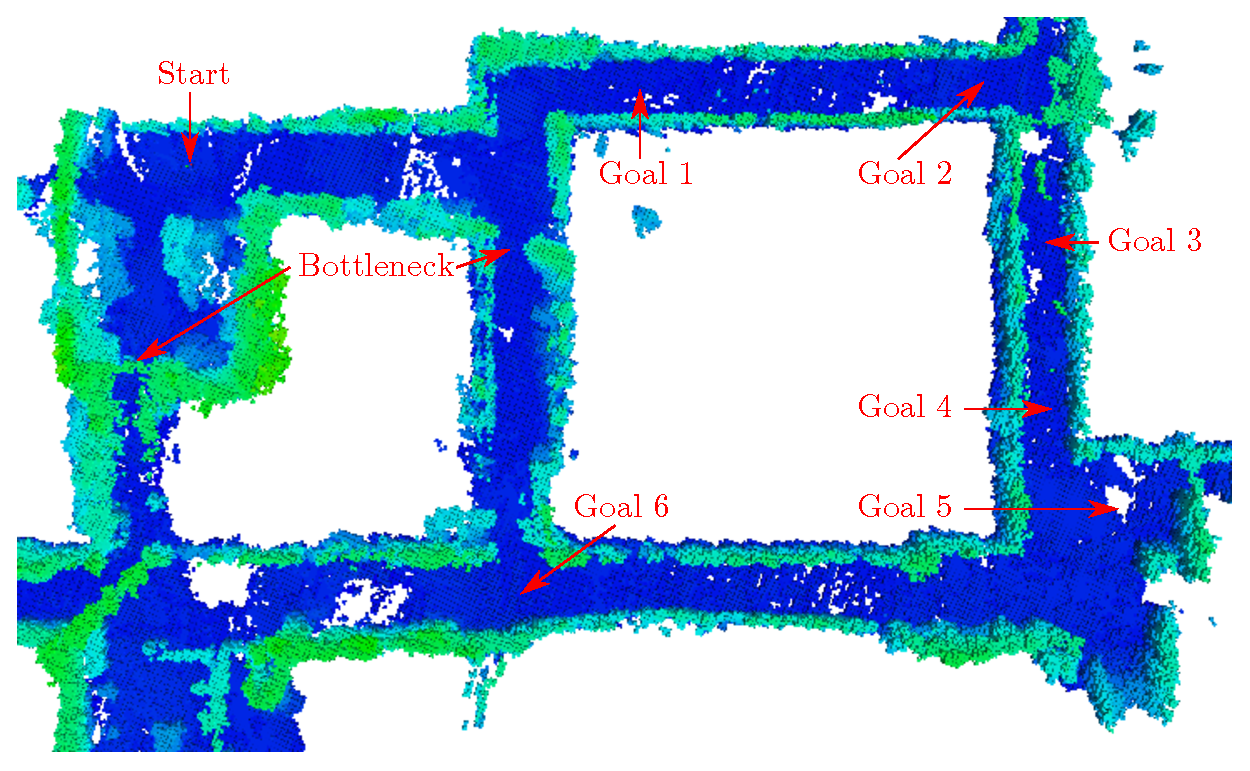
\includegraphics[trim = 0mm 15mm 0mm 0mm,clip,width=1\textwidth]{pics/ML4.eps}
   \caption{Bird's eye perspective on hallways in the "ML" building of the ETH Zurich. One start vertex and 6 different goal vertices are depicted}
   \label{pic:differentGoal}
\end{figure}

%\begin{figure}[h]
%   \centering
%   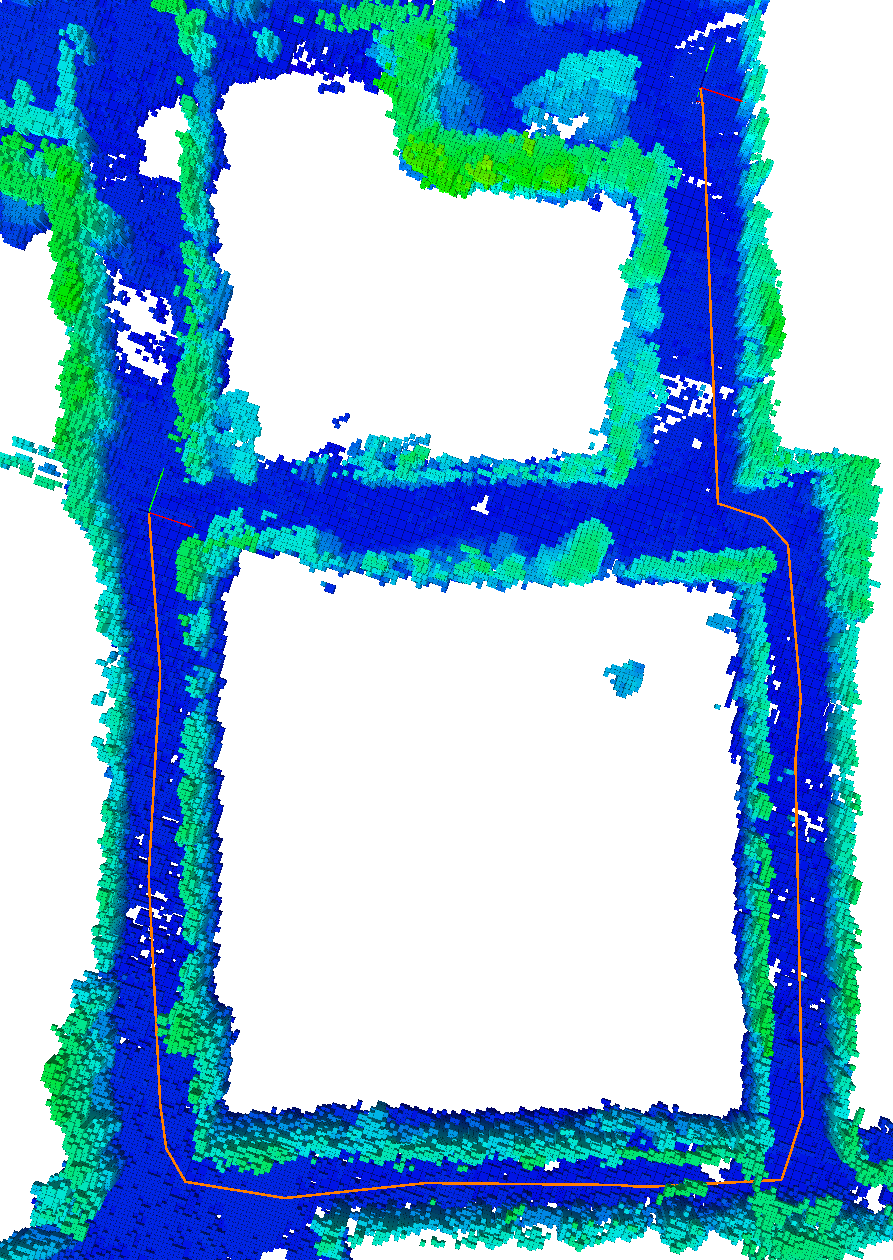
\includegraphics[width=0.5\textwidth]{pics/MapLine.png}
%   \caption{Ein Bild.}
%\end{figure}
%
%
%\begin{figure}[h]
%   \centering
%   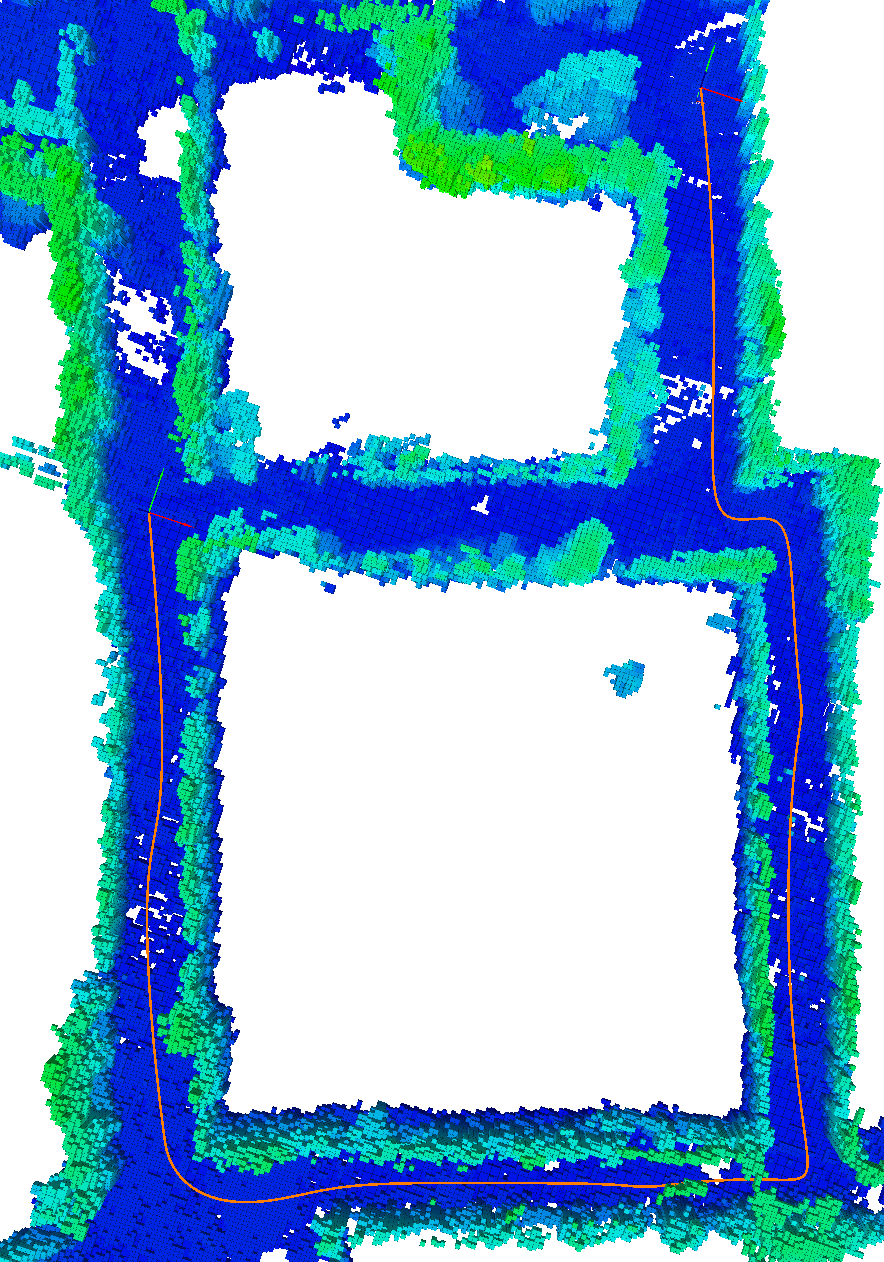
\includegraphics[width=0.5\textwidth]{pics/MapPoly.png}
%   \caption{Ein Bild.}
%\end{figure}

The bottleneck in the center of figure \ref{pic:differentGoal} gets significant for large bounding boxes. If the dimension of the bounding box are larger than $0.5m$ x $0.5m$ x $0.5m$ the trajectory is not able to pass the bottleneck. Hence, a trajectory with a large bounding box has to go all the way around to proceed from the start vertex to "Goal 6" as depicted in figure \ref{pic:Goal6}.


\begin{figure}[H]
   \centering
   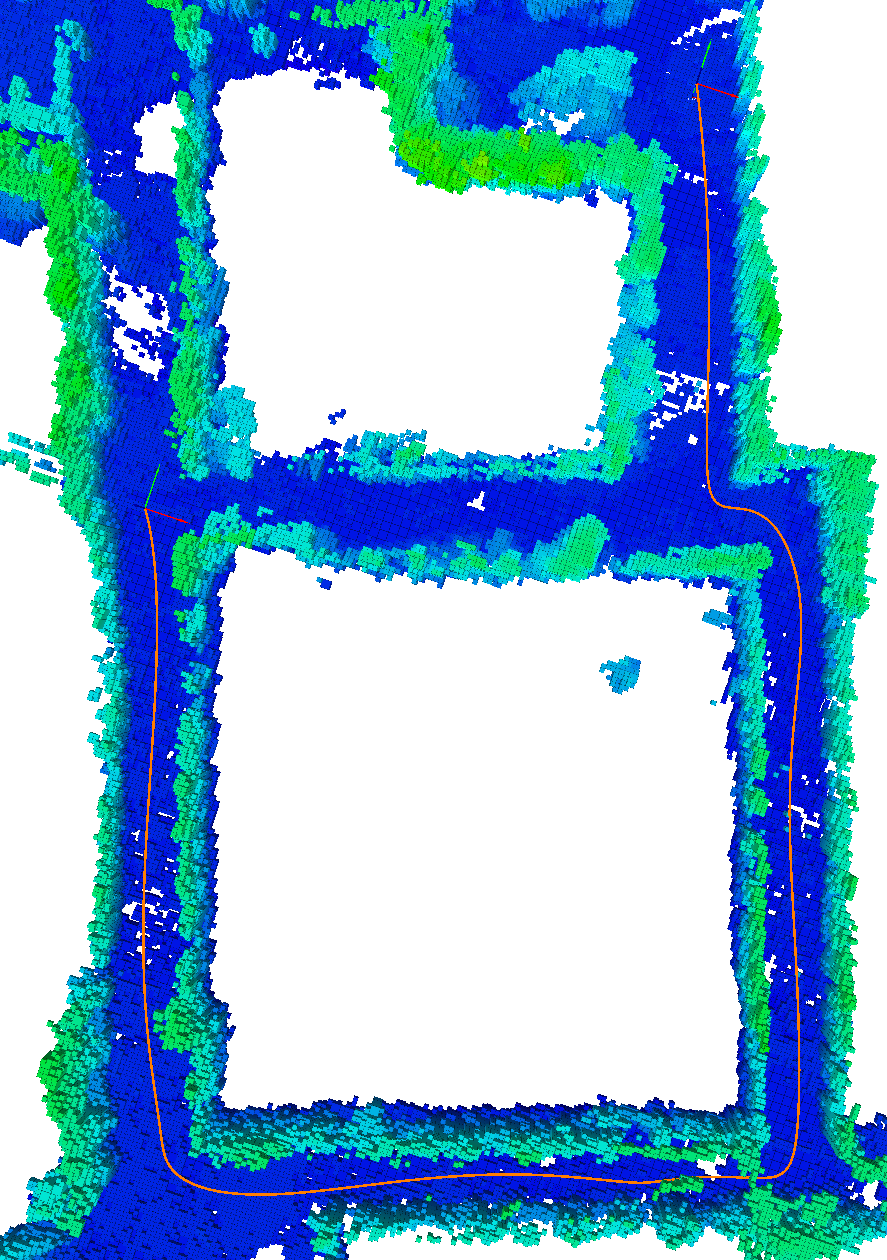
\includegraphics[angle=90,trim = 20mm 0mm 0mm 0mm,clip, width=1\textwidth]{pics/MapNlopt.png}
   \caption{Trajectory from the start vertex to "Goal 6". Due to the bottleneck in the hallway in the middle, the trajectory has to proceed all the way around.}
   \label{pic:Goal6}
\end{figure}

The trajectories from the start vertex to the 6 different goal vertices (depicted in figure \ref{pic:differentGoal}) are examined for number of segments and the duration of NLopt. The only ending criteria for NLopt was the relative criteria on the total cost $f_{rel} = 0.02$. 
In addition to the number of segments, the number of corresponding optimization variables (endpoint derivatives $d_p$ and segment times $T_i$) are calculated. For all the "free" vertices (which are neither the start nor the goal vertex) there are 12 optimization variables, namely the velocity, the acceleration, the jerk and the snap in the 3 dimensions. Furthermore, the segment times are optimization variables. \newline

Since the number of free vertices is the number of segment $n_{seg}$ minus 1, the equation for the number of optimization variables $n_{var}$ is:

\begin{equation}
n_{var} = (n_{seg} - 1)\cdot 12 + n_{seg}
\label{equ:numberOfSeg}
\end{equation}

The results for the 6 different goal vertices are listed in the following table:


\begin{table}[H] 
\begin{center}
    \begin{tabular}{| c | c | c | c | }
    \hline
    Goal Vertex & Segments & Optimization Variables & Optimization Time\\ \hline
   Goal 1 & 5 & 53 & $1.15s$\\ \hline
  Goal 2 & 8 & 92 & $2.94s$\\ \hline
   Goal 3 & 11 & 131 & $7.80s$\\ \hline
Goal 4 & 15 & 183& $42.96s$\\ \hline
Goal 5 & 19 & 235& $93.08s$\\ \hline
   Goal 6& 20 & 248 & $347.62s$\\
    \hline
    \end{tabular}
    \caption{The number of segments of the collision free polynomial solution and the corresponding number of optimization variables. The time needed by NLopt with the ending criteria $f_{rel} = 0.02$.}
    \label{tab:MLoptimizationTime}
\end{center}
\end{table}

Table \ref{tab:MLoptimizationTime} shows that the optimization time (i.e. the duration of the NLopt algorithm) increases significant for a large amount of optimization variables. Comparing the result of "Goal 5" to "Goal 6" it becomes clear, that the number of optimization variables is not the only factor which determines the optimization time. If the optimization values of the initial solution are close to the global minimum of the cost function, the optimization takes less time and vice versa. Still, the number of optimization variables is the main factor. \newline

Please note that the RRT* algorithm was only executed once for every goal vertex. Due to the randomness of the RRT* algorithm, the number of segments could change for unchanged start and goal vertices.\newline



\section{Reduction of the Optimization Variables}

The results in table \ref{tab:MLoptimizationTime} have shown, that the performance of NLopt decreases with a large amount of optimization variables. In cases where the optimization times is significant (i.e. online planning) the number of optimization parameters has to be reduced. The benefits and the drawbacks of a cost function with fewer optimization variables is discussed in the next section. \newpage

\subsection{Cost Function Without Endpoint Derivatives}

To call to mind, the cost function for the nonlinear optimization is 

\begin{equation}
J_{total} =
\begin{bmatrix}
   d_f \\
  d_p
\end{bmatrix}^T
\begin{bmatrix}
   R_{ff} & R_{fp} \\
  R_{pf} & R_{pp}
\end{bmatrix}
\begin{bmatrix}
   d_f \\
  d_p
\end{bmatrix}
+ k_T \cdot \sum_{i=1}^N T_i
\label{equ:total_cost_Result}
\end{equation}

where the optimization variables are the segment times $T_i$ and the unspecified endpoint derivatives $d_p$. $k_T$ is a user specified weighting factor and $d_f$ is the vector containing the fixed endpoint derivatives. The 4 sub-matrices of $R$ are containing the quadratic snap rearranged according to the fixed and unspecified endpoint derivatives. \newline
As discussed in section \ref{sec:nonlinearopt}, the optimum of this cost function can not be found analytically but with a nonlinear optimization. Only the snap minimized solution of a trajectory with fixed segment times can be computed analytically according to 



\begin{equation}
d_p^* = - R_{pp}^{-1} \cdot R_{fp}^T \cdot d_f
\label{equ:dpstar_Result}
\end{equation}

where the optimal unspecified endpoint derivatives  $d_p^*$ are a function of the fixed derivatives $d_f$ and two of the submatrices ($R_{pp}, R_{fp}$) of $R$. \newline

Since the endpoint derivatives $d_p$ can be found analytically once the segment times $T_i$ are known, $d_p$ can be excluded from the optimization variables. In other words, in every optimization steps the segment times are modified by NLopt. Then $d_p^* $ is computed with the current segment times and the total cost is calculated according to equation \ref{equ:total_cost_Result}. \newline

Recapitulating the new cost function:

\begin{itemize}
  \item The segment times $T_i$ are the only optimization variables.
  \item The optimal unspecified endpoint derivatives $d_p^*$ are computed analytically (equation \ref{equ:dpstar_Result}) every optimization step with the current segment times.
    \item The cost function (equation \ref{equ:total_cost_Result}) gets minimized.
\end{itemize}

\subsection{Comparison of the Analytical Solvers}

Before we can compare the performance of the approach with the full number of optimization variables (in the interests of simplification called approach A) to the approach with the reduced number of optimization variables (approach B) we have to examine the performance of the analytical solver which solves equation \ref{equ:dpstar_Result}.\newline

An analytical or linear solver is able to solve an single matrix equation:

\begin{equation}
A \cdot x = b
\label{equ:linearSolver}
\end{equation}


Indeed, equation \ref{equ:dpstar_Result} is a single matrix equation where $-R_{pp}$ is represented by $A$ and $x$ is the vector containing the optimization variables (i.e. $d_p$). Furthermore, $R_{fp}^T \cdot d_f$ can be taken together as vector $b$. \newline

In this master thesis, three different strategies have been implemented to solve equation \ref{equ:dpstar_Result}.
All of them are part of "Eigen". Eigen is a C++ template library for linear algebra: matrices, vectors, numerical solvers, and related algorithms. The definition of the implemented strategies can be found on the  \href{http://eigen.tuxfamily.org/index.php?title=Main_Page}{Eigen-homepage} \cite{Eigen}:

\newpage

\subsubsection{FullPivLU}

This class represents a $LU$ decomposition of any matrix, with complete pivoting: the matrix $A$ is decomposed as $A = PLUQ$ where $L$ is unit-lower-triangular, $U$ is upper-triangular, and $P$ and $Q$ are permutation matrices. This is a rank-revealing $LU$ decomposition. The eigenvalues (diagonal coefficients) of $U$ are sorted in such a way that any zeros are at the end. \newline

$FullPivLU$ is a very accurate technique but rather slow.

\subsubsection{HouseholderQR}

This class performs a $QR$ decomposition of a matrix $A$ into matrices $Q$ and $R$ such that $A = QR$ by using Householder transformations. Here, $Q$ a unitary matrix and $R$ an upper triangular matrix. The result is stored in a compact way compatible with $LAPACK$. Note that no pivoting is performed. This is not a rank-revealing decomposition.\newline

$HouseholderQR$ is a fast technique but in general less accurate than $FullPivLU$.

\subsubsection{Inverse}
For small fixed sizes up to $4x4$, this method uses cofactors. In the general case, this method uses class $PartialPivLU$. This class represents a $LU$ decomposition of a square invertible matrix, with partial pivoting: the matrix $A$ is decomposed as $A = PLU$ where $L$ is unit-lower-triangular, $U$ is upper-triangular, and $P$ is a permutation matrix. \newline

The performance of the inverse is compared experimentally to the other techniques. \newline

First, the three techniques were tested with a long trajectory. The initial solution has been computed for a trajectory with 300 segments with random vertices. The identical set of vertices was used for all the three techniques and the results are listed in the following table:

\begin{table}[H] 
\begin{center}
    \begin{tabular}{| c | c | }
    \hline
    Technique & Computational Time  \\ \hline
  FullPivLU  & $19.52s$\\ \hline
  HouseholderQR & $3.34s$\\ \hline
 Inverse & $2.07s$\\
    \hline
    \end{tabular}
    \caption{Comparison of the three analytical solvers for a trajectory with 300 segments. Only the initial solution has been computed.}
    \label{tab:300seg}
\end{center}
\end{table}

In a next step, the three techniques has been compared in the nonlinear optimization. The RRT* algorithm was executed to find a straight lines solution from the start vertex to "Goal 6" in figure \ref{pic:differentGoal}. The collision-free polynomial trajectory had 23 segments. The trajectory was optimized using $FullPivLU$ but in every iteration $HouseholderQR$ and $Inverse$ has been computed as well and the total time of the individual techniques has been stored. The optimization terminated after 883 iterations. \newpage

The result of the three techniques are listed in the following table:

\begin{table}[H] 
\begin{center}
    \begin{tabular}{| c | c | }
    \hline
    Technique & Computational Time  \\ \hline
  FullPivLU  & $1.134s$\\ \hline
  HouseholderQR & $0.704s$\\ \hline
 Inverse & $0.285s$\\
    \hline
    \end{tabular}
    \caption{Comparison of the three analytical solvers for a trajectory with 23 segments. The nonlinear optimization was performed (883 iterations).}
    \label{tab:883iter}
\end{center}
\end{table}

As mentioned above $FullPivLU$ is very accurate. In the two above noted tests (and also in other performed tests) the other two techniques led to the same result as $FullPivLU$, meaning there were no numerical stability issues. This is due to the fact, that $R_{pp}$ is quadratic and a band matrix. A band matrix is a sparse matrix whose non-zero entries are confined to a diagonal band. Band matrices are beneficial from a computational point of view. \newline

Since the numerical stability is given for all of the techniques the determining factor is the computational time. Therefore, the $Inverse$ is the preferable technique! \newline

Please note that the $FullPivLU$ and $HouseholderQR$ have to solve equation \ref{equ:dpstar_Result} separate for each dimension. In contrast, the inverse has to be computed once and can then be applied to the three dimensions. This means that $HouseholderQR$ would be faster than $Inverse$ if only on dimension had to be optimized. However, in this master thesis with three dimension the inverse can display his advantages.


\subsection{Comparison of the Different Approaches}

Table \ref{tab:MLoptimizationTime} depicts the optimization time from the start vertex to "Goal 6" using the approach with the full number of optimization variables (approach A). Table \ref{tab:883iter} depicts the computational time for the same start and goal vertex using the approach with the reduced number of optimization variables (approach B). Caution, the time needed for the limit check $v_{max}$ and $a_{max}$ is not included in table \ref{tab:883iter}. \newline 

Although the number of segments are slightly different (based on the randomness of RRT*) and table \ref{tab:883iter} does not include the time needed for the limit check it is obvious that approach B with a computational time of $0.285s$ is much faster than approach A with a optimization time of $347.62s$.\newline 


During the further procedure of comparing the two approaches, the focus is on the final trajectory cost.
As a consequence of the reduction of the optimization variables, approach B is not able to reach the global minimum of the cost function in all cases. Approach A on the other hand, is theoretical allays able to reach the global minimum of the cost function. In practice, depending on the initial values and on the ending criteria, it happens that the optimization only finds a local minimum. The performance of the two strategies has therefore to be testes experimentally. \newline

Here comes the comparison!!!!!

\newpage


%\section{Performance of the RRT* Algorithm}
%
%In this master thesis, the performance of the RRT* algorithm itself was not improved but the parameters were tuned to serve the nonlinear optimization in an optimal manner.
%
%As mentioned in section \ref{sec:RRTstar}, the calculation time of the RRT* algorithm is mainly defined by the "rewiring" and therefore by the user specified parameter $\gamma$ (used in equation \ref{equ:ballradius}). A good straight line solution, whereas good means a small length of the straight line solution, does not necessarily lead to a good polynomial trajectory. The influence of the user specified parameter $\gamma$ on the final trajectory and the corresponding calculation time is evaluated in this section. \newline
%Please call to mind that a small $\gamma$ parameter means little rewiring and a big $\gamma$ parameter means lots of rewiring. The impact of the $\gamma$ parameter can be looked up in figure \ref{pic:smallGamma} and figure \ref{pic:smallBBX}.\newline
%
%Figure \ref{pic:boxplot} depicts the boxplot for different $\gamma$ parameters. Each dataset consists of 15 measurements. On each box, the central mark is the median, the edges of the box are the 25th and 75th percentiles, the whiskers extend to the most extreme
%datapoints the algorithm considers to be not outliers, and the outliers are plotted individually. 
%
%
%\begin{figure}[H]
%   \centering
%   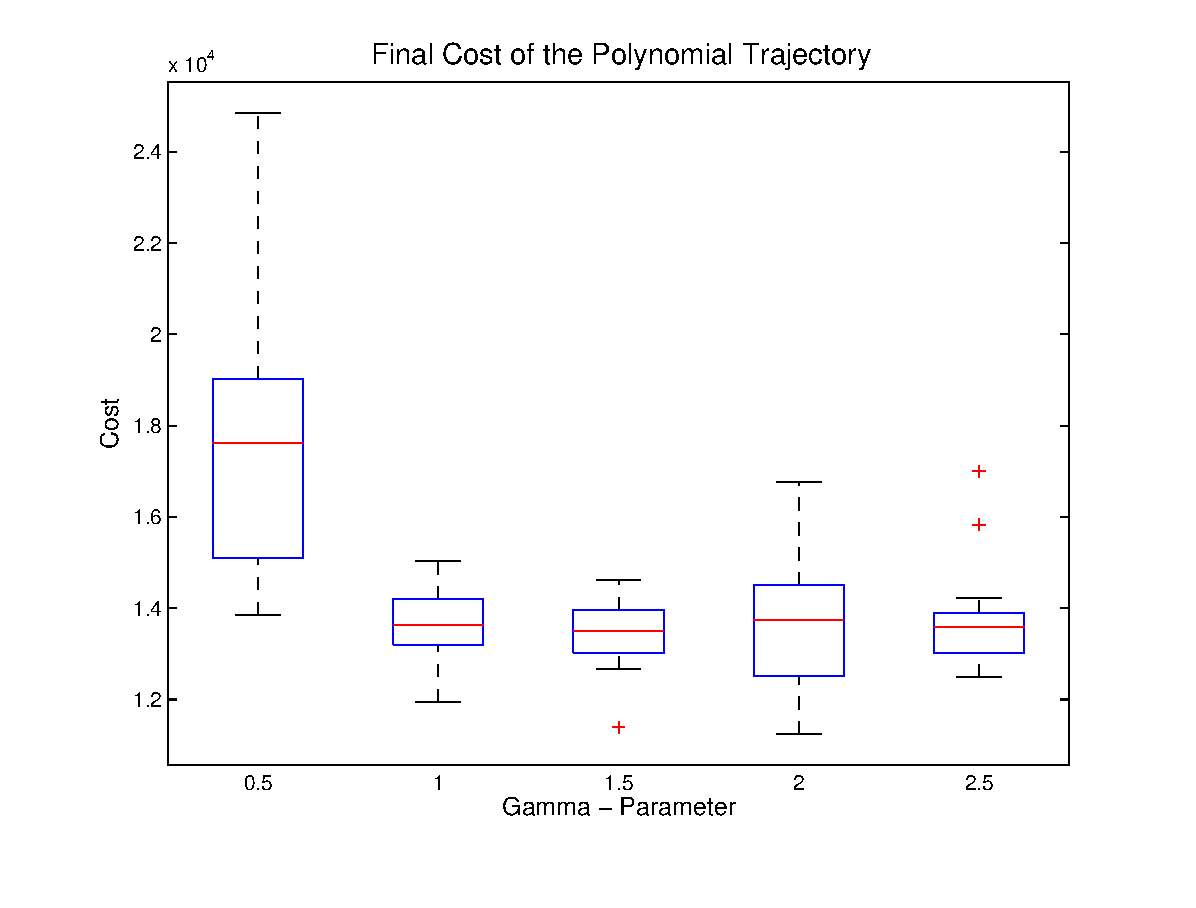
\includegraphics[trim = 14mm 10mm 15mm 0mm,clip,width=1\textwidth]{pics/boxplot1.eps}
%   \caption{The $x$-axis depicts different $\gamma$ parameters and the $y$-axis depicts the final cost of the polynomial trajectory. The red mark illustrates the median. }
%   \label{pic:boxplot}
%\end{figure}
%
%
%It becomes apparent that the small amount of rewiring associated with $\gamma = 0.5$ is to little to obtain a good polynomial trajectory. The 4 remaining datasets have a similar performance in terms of the final trajectory cost. \newline
%
%The total computational times for the five different $\gamma$ parameters are depicted in figure \ref{pic:boxplot_time}. The total computational time is the combined duration of the RRT* algorithm and the nonlinear optimization.  In contrast to the final cost, the total computational times for $\gamma = 1 $, $\gamma = 1.5$, $\gamma = 2$ and $\gamma = 2.5$ are distinct. 
%
%\begin{figure}[H]
%   \centering
%   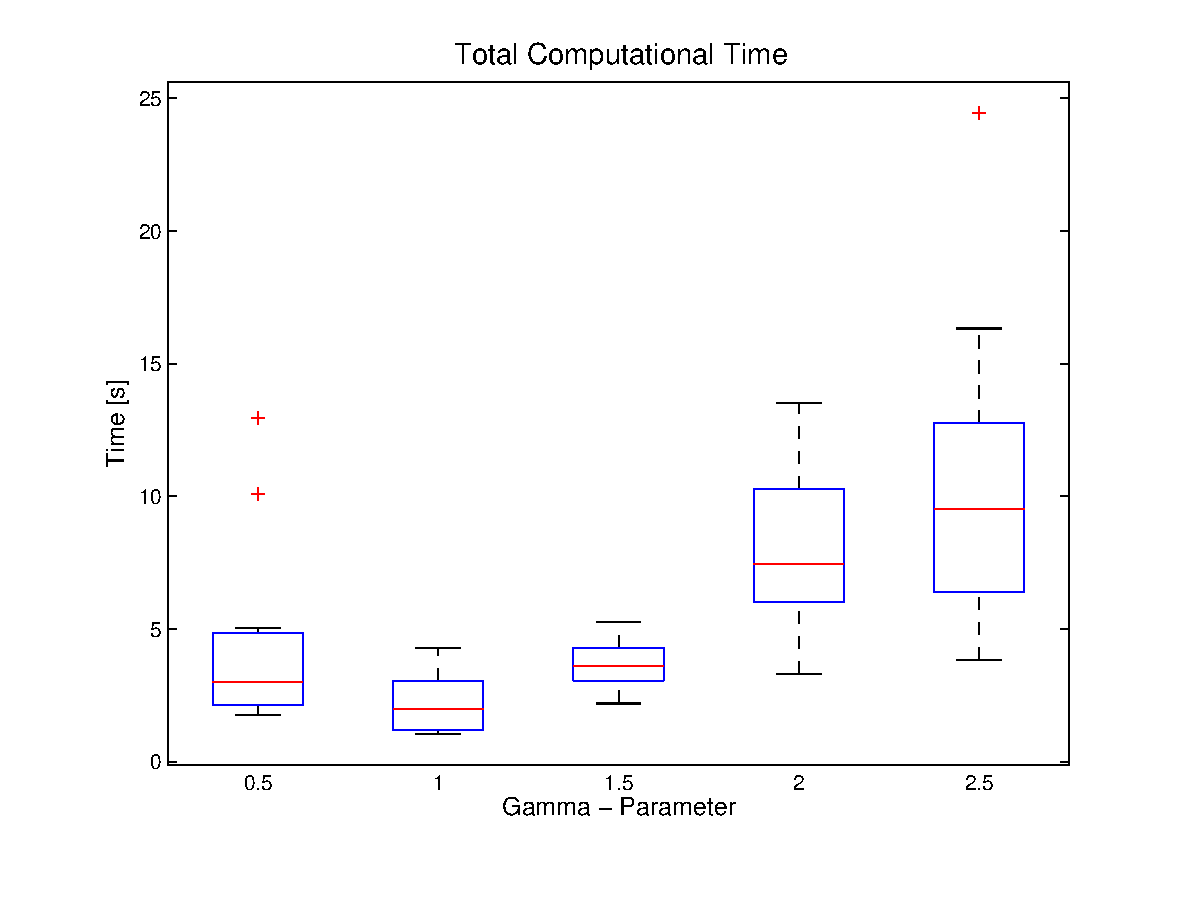
\includegraphics[trim = 14mm 10mm 15mm 0mm,clip,width=1\textwidth]{pics/boxplot_time.eps}
%   \caption{The $x$-axis depicts different $\gamma$ parameters and the $y$-axis depicts the total computational time. The red mark illustrates the median.}
%   \label{pic:boxplot_time}
%\end{figure}
%
%Figure \ref{pic:boxplot_time} shows that the computational time increases significant if $\gamma$ is larger than 1.5. This is simply because the RRT* algorithm needs more time for rewiring. Furthermore, $\gamma = 0.5$ (which is not a good choice sine the final cost is too high) has 2 outliers. In this 2 cases the straight line solution is not enough target-orientated and multible vertex extensions are required to obtain a collision-free trajectory. \newline
%
%Combining the results from figure \ref{pic:boxplot} and figure \ref{pic:boxplot_time}, a $\gamma$ parameter in the range of 1 to 1.5 lead to the best performance.




%
%\begin{figure}
%\centering
%\begin{subfigure}{.5\textwidth}
%  \centering
%  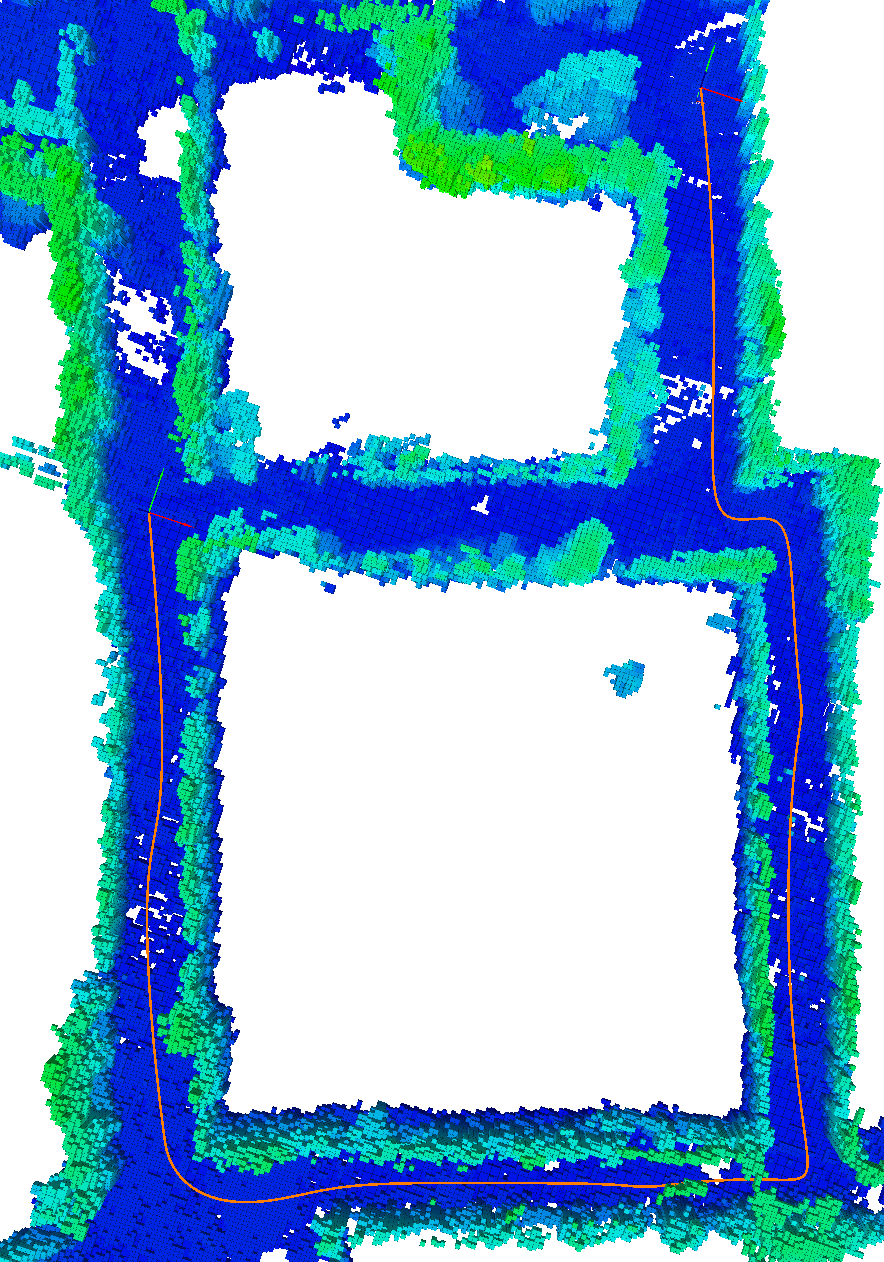
\includegraphics[width=1\linewidth]{pics/MapPoly.png}
%  \caption{A subfigure}
%  \label{fig:sub1}
%\end{subfigure}%
%\begin{subfigure}{.5\textwidth}
%  \centering
%  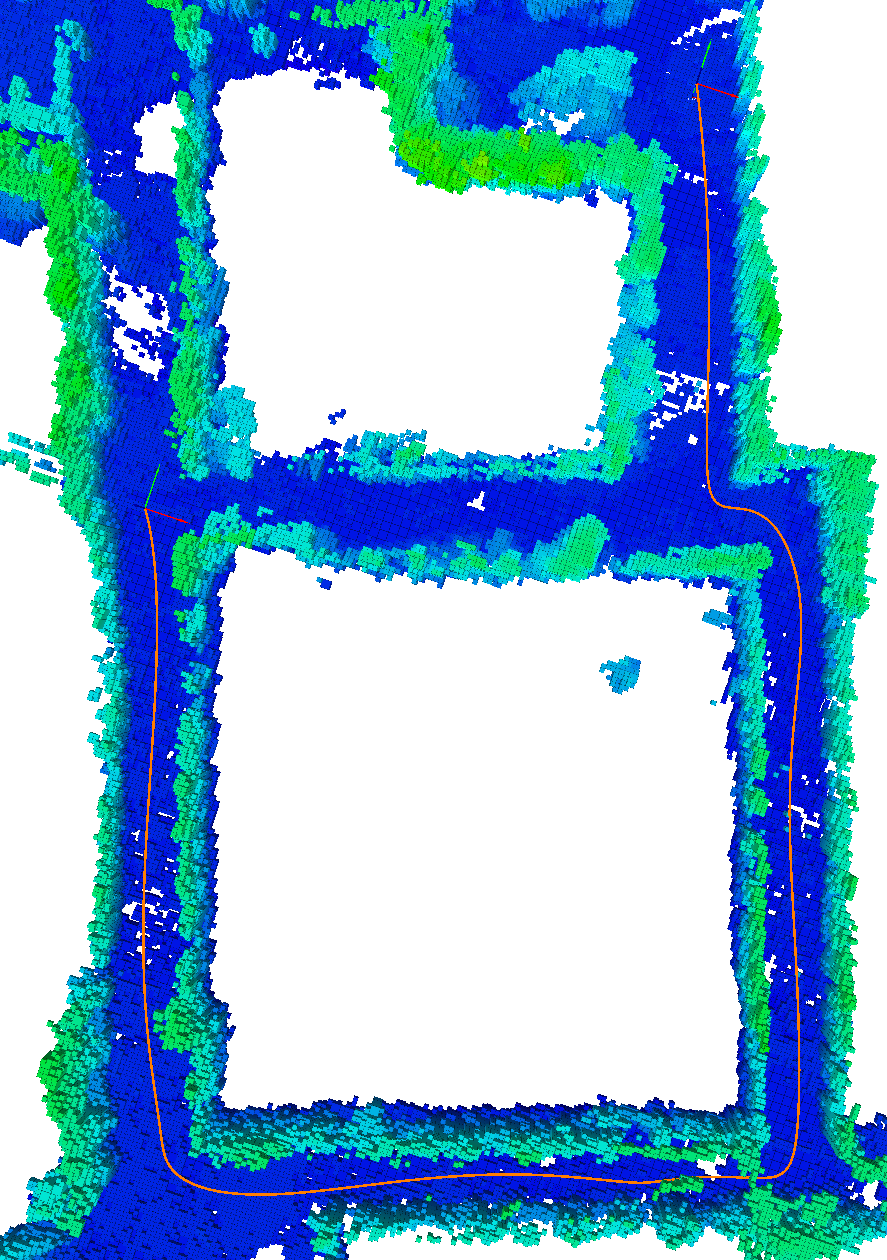
\includegraphics[width=1\linewidth]{pics/MapNlopt.png}
%  \caption{A subfigure}
%  \label{fig:sub2}
%\end{subfigure}
%\caption{A figure with two subfigures}
%\label{fig:test}
%\end{figure}

